\documentclass[sigconf,natbib=true]{acmart}
%-------------------------------------------------------------------------------
% PACKAGES FOR THE TEXT TYPE
%-------------------------------------------------------------------------------
\usepackage[english]{babel}
\usepackage[utf8]{inputenc}
\usepackage[T1]{fontenc}
%-------------------------------------------------------------------------------
% FOR FIGURES AND CAPTIONS
%-------------------------------------------------------------------------------
\usepackage{graphicx,graphics,float,subcaption,wrapfig,epstopdf}
\epstopdfsetup{update}
\usepackage[labelfont=bf]{caption} 
%------------------------------------------------------------------------------
% FOR CHECKMARK
%-------------------------------------------------------------------------------
\usepackage{tikz}
\def\check{\tikz\fill[scale=0.3](0,.35) -- (.25,0) -- (1,.7) -- (.25,.15) -- cycle;} 
%-------------------------------------------------------------------------------
% FOR TABLE COLUMNS
%-------------------------------------------------------------------------------
\usepackage{array} 
\newcolumntype{L}[1]{>{\raggedright\let\newline\\\arraybackslash\hspace{0pt}}m{#1}}
\newcolumntype{C}[1]{>{\centering\let\newline\\\arraybackslash\hspace{0pt}}m{#1}} 
\newcolumntype{R}[1]{>{\raggedleft\let\newline\\\arraybackslash\hspace{0pt}}m{#1}}
%\NewDocumentCommand{\rot}{O{80} O{1em} m}{\makebox[#2][l]{\rotatebox{#1}{#3}}}%
\usepackage{multirow, makecell}
%\usepackage{booktabs} % To thicken table lines
%-------------------------------------------------------------------------------
% PACKAGES FOR URL
%-------------------------------------------------------------------------------
%\usepackage[hyphens]{url}
\usepackage{hyperref}
\usepackage{breakurl}
\hypersetup{colorlinks, citecolor=blue, filecolor=blue, linkcolor=blue,urlcolor=blue}
%-------------------------------------------------------------------------------
% FOR ACRONYMS 
%-------------------------------------------------------------------------------
\newcommand{\eg}{\textit{\mbox{e.g.,~}}} 
\newcommand{\ie}{\textit{\mbox{i.e.,~}}} 
\newcommand{\et}{\textit{\mbox{et al.~}}}

%-------------------------------------------------------------------------------
% VARIABLES
%-------------------------------------------------------------------------------
\newcommand{\DDOSDBMULTIVECTORKEYS}{????~}
\newcommand{\DDOSDBINSTANCES}{????~}
\newcommand{\PROTECTEDORGANISATIONS}{????~}

%-------------------------------------------------------------------------------
% COPYRIGHT
%-------------------------------------------------------------------------------
\renewcommand\footnotetextcopyrightpermission[1]{} % removes footnote with conference info
\setcopyright{none}
%\setcopyright{acmcopyright}
%\setcopyright{acmlicensed}
%\setcopyright{rightsretained}
%\setcopyright{usgov}
%\setcopyright{usgovmixed}
%\setcopyright{cagov}
%\setcopyright{cagovmixed}

\settopmatter{printacmref=false, printccs=false, printfolios=false}

% DOI
\acmDOI{}

% ISBN
\acmISBN{}

%Conference
%\acmConference[Submitted for review to SIGCOMM]{}
%\acmYear{2018}
%\copyrightyear{}

%% {} with no args suppresses printing of the price
\acmPrice{}

%------------------------------------------------------------------------------
%------------------------------------------------------------------------------
\begin{document}
%------------------------------------------------------------------------------
% TITLE
%------------------------------------------------------------------------------
\title{Solving DDoS Attacks\\by Standing on the Shoulders of Giants}
\subtitle{DDoS Clearing House, DDoSDB, DDoS Dissector, DDoS Fingerprint and Converters}
\titlenote{This document was not peer-reviewed.}
%------------------------------------------------------------------------------
% AUTHORS
%-------------------------------------------------------------------------------
% \author{Paper \# XXX, XXX pages}
%\author{Jair Santanna}
%\affiliation{\institution{University of Twente}  \streetaddress{The Netherlands}}
%\email{j.j.santanna@utwente.nl}
%
%\author{Koen van Hove}
%\affiliation{\institution{University of Twente}	\streetaddress{The Netherlands}}
%\email{k.w.vanhove@student.utwente.nl}


%\author{João Ceron}
%\affiliation{\institution{University of Twente}	\streetaddress{The Netherlands}}
%\email{j.m.ceron@utwente.nl}

%\author{Aiko Pras}
%\affiliation{\institution{University of Twente}	\streetaddress{The Netherlands}}
%\email{a.pras@utwente.nl}

%\author{Cristian Hesselman}
%\affiliation{\institution{SIDN Labs}	\streetaddress{The Netherlands}}
%\email{cristian.hesselman@sidn.nl}

%% The default list of authors is too long for headers}
%\renewcommand{\shortauthors}{Santanna et al.}
%------------------------------------------------------------------------------
% ABSTRACT
%-------------------------------------------------------------------------------
%\begin{abstract}
    .
\end{abstract}
\maketitle
%------------------------------------------------------------------------------
% SECTIONS
%-------------------------------------------------------------------------------
\section{Introduction}
\label{introduction}

Distributed Denial of Service attacks exist since the beginning of the Internet. The goal of these types of attacks is to make target systems (services, devices, or even entire networks) unreachable to its intended users. Over time, these types of attacks increased in frequency and intensity. In 2011, the peak record was reported as 60Gb/s~\cite{}, in 2015 it was 500Gb/s~\cite{}, and in 2016 was 1.1Tb/s~\cite{}. As the dependency of our society to online service also increased, the damage cause by DDoS attacks has become extremely big.  While in 2015 large corporations reported the average loss of \$US410.000 per attack~\cite{}, in 2017 this figure increased to \$US2.500.000~\cite{}.

There are hundreds of companies worldwide offering DDoS protection and a large volume of academic work on DDoS attacks. Overall, DDoS attacks have been addressed as a reactive approach, waiting for attacks to hit a network infrastructure and see whether (i) the usual anomaly-based detection/mitigation solution works, or (ii) the network operators are skilled enough to mitigate the attack as fast as possible, or (iii) by simply paying more to third-party companies for having more network capacity and better protection. From the academic side, by the end of February 2019, Google scholar returned more than 47 thousand works on ‘ddos attack’. 

The question that we intend to discuss in this paper is \textbf{why and how (we believe), together, we can solve DDoS attacks?} The answer is technically simply and it is \textbf{not} by ``reinventing the wheel'', instead, facilitating filling the gaps of existing solutions and stakeholders (\eg victims, network operators, network security community, network security companies, law enforcement agencies, and the academic community). What we propose is a proactive approach that any stakeholder involved with a DDoS attack would benefit and trust.

Overall, we propose to facilitate: (1) victims, (2) network operators, and (3) network security companies to share their attack measurements (filtered and properly anonymized) and to get in return specific rules for detecting and mitigating those attack based on the already in-place solutions; (4) law enforcement agencies to compare attacks suffered in the society, for enabling legal attribution and prosecution of attackers (and buyers of attacks); (5) network security community (specially CERT/CSIRT) to get frequent feeds with IP addresses involved in attacks, towards preventing misused machines from performing attacks; and (6) the academic community on getting real/`fresh' DDoS attack data for testing and improving their solutions. For satisfying these six stakeholders, we propose and extensively validate the following three elements: 

\begin{itemize}
	\item \textbf{DDoS Dissector}: is a tool for analysing any type of network trace containing a DDoS attack (for example, pcap, pcapng, neflow, ipfix, sflow, and apache log), filter only the main characteristics of the attack, called \textbf{DDoS fingerprint}, and enable to share only the DDoS fingerprint and the anonymized version of the filtered attack. The requirements, the design and the validation of the tool is presented at \autoref{sec:ddos_dissector}; %100\% true positive
	
	\item\textbf{DDoS Fingerprint Converters}: is a set of tools for parsing the generic DDoS fingerprints into specific detection and mitigation technologies, for example, BGP Flowspec, eBPF, IPtables, SNORT, SURICATA, BRO, ModSecurity, and even ‘black-boxes’ from private security companies. An additional, and very important tools added to this set of converters, called \textbf{DDoS Mitigation Impact Quantification}, is responsible to validate and adapt detection and mitigation rules. The descriptions and explanations are presented at \autoref{sec:fingerprint_converters};
	
	\item \textbf{DDoS Database (DDoSDB)}: is a distributed database that receives, enriches, distributes, and make available: filtered anonymized attack traces, DDoS fingerprints, signatures/rules for specific hardware/software detecting/mitigating DDoS attacks, lessons learned from network operators, information from law enforcement agencies and feeds for CERT/CSIRT sanitize their networks. The requirements, the design and the validation of the tool is presented at \autoref{sec:ddosdb}.
\end{itemize}

After we describe the DDoS Dissector, the DDoS Fingerprint Converters, and the DDoS Database (DDoSDB), we introduce what we call as \textbf{DDoS Clearing House} in \autoref{sec:ddos_clearinghouse}. Only at that point we put all the pieces together and show how we have deployed \DDOSDBINSTANCES instances of the DDoSDB, collected more than \DDOSDBMULTIVECTORKEYS, and benefit more than \PROTECTEDORGANISATIONS organizations. The development of the tools are available at \url{https://github.com/ddos-clearing-house} and the public version of DDoSDB is available at \url{https://ddosdb.org}.


%Distributed Denial of Service (DDoS) attacks \citep{}
%
%Why standing on the shoulders of gigants: existing solutions and stakeholders. Not reinvent the wheel but adding 
%
%The solutions against DDoS attacks are based on technologies (hardware and software) that monitors the network traffic and react upon a predefined event. There are mainly two types of events. The first is when occurs a match between the incoming network traffic (packet or flow) and a predefined rule or signature, called rule/signature-based Intrusion Prevention System (IPS). The second type of event is when the network traffic has an abnormal behaviour based on a predefined profile. This latter type of technology is called anomaly-based IPS. 
%
%An ideal scenario for the mitigation of a DDoS attack would be a distributed solution with a r connected to an anomaly-based IPS.
%
%Different types of attacks requires different types of mitigation strategy.
%
%The difference between an intrusion detection systems (IDS) and an  is that the latter can launch an action after a detection event, while the former records an event after the detection. Sometimes these terms are interchangeable by the community.
%
%There are two types of IDS/IPS: signature and anomaly-based. While the signature-based IPS is 
%
%For us, the DEFINITION of a DDoS fingerprint is an useful comprehensive summary of the characteristics of a single vector of a DDoS attack extracted from a network measurement.
%
%*misunderstanding digital fingerprint, signature, rule, pattern, characteristics, profile
%
%Law enforcement agencies do not like to call \emph{digital fingerprint} because in their field a fingerprint leads to an unique individuo.
%
%THE PROBLEM can be summarized as: (1) a lack of standard for fingerprinting DDoS attacks; (2) lack of an updated database with fingerprints; (3) lack of functions to convert DDoS fingerprints into applicable detection and mitigation rules; 
%
%Rule-based mitigation solutions (\eg firewall, BGP flowspec,) are an particular case of signature-based IDS.
%
%Types of network measurements are: (1) packet-based (\ie pcap and pcapng), (2) (net)flow-based (\eg v5, v9, IPFIX), (3) sflow, and (3) log-based. 
%
%USAGE of the fingerprint: (1) improve existing detection and mitigation solutions, (2) attribution, (4) correlation among DDoS attacks and correclaation with other types of cyber threats, (5) accounting for attacks, and (6) notification to CSIRT/CERT's for cleaning misused machines, (3) facilitate the access to attacks traffic (usually for academic purpose)
%
%Detection and mitigation tools for DDoS attacks: (1) BGP Flowspec, (2) BRO, (3) SURICATA, (4) SNORT, (5) ModSecurity, (6) eBPF, (7) IPtables.
%
%Unicast addresses
%
%How much is needed to be collected (time, packets, flows)? 
%How much is the impact of a mitigation rule (considering the ongoing traffic)?
%How to indicate spoofed IP presence?
%
%% Enrichments: AS, geolocation, open ports, spoofed?, blacklisted?,
%
%We intend to solve the problem that DDoS attacks pose by ...
%
%DDoS attacks are not likely to stop happening!




\section{DDoS Dissector}
\label{sec:ddos_dissector}
%about fingerprint: concepts \& context}

There are several words used in academia and the security community for what we will define as a DDoS attack fingerprint. The words are DDoS `characteristics', `fingerprint', `profile', `pattern', `signature', and `rule'. Oxford dictionary defines these words as the following:

\begin{itemize}
	\item \textbf{characteristics}: ``a feature or quality belonging typically to a person, place, or thing and serving to identify them'';
	\item \textbf{profile}: ``a graphical or other representation of information relating to particular characteristics of something, recorded in quantified form'';
	\item \textbf{pattern}: ``a regular and intelligible form or sequence discernible in the way in which something happens or is done'';
	\item \textbf{signature}: ``a distinctive pattern, product, or characteristic by which someone or something can be identified'';
	\item \textbf{rule}: ``a principle that operates within a particular sphere of knowledge, describing or prescribing what is possible or allowable'';
\end{itemize}

We will however use an umbrella term, a \textbf{fingerprint}, from which the above five can be derived. A fingerprint is the smallest set of features that summarizes the main characteristics of each attack vector in a DDoS attack, extracted from a network measurement of the attack.

The goal of determining the fingerprint is to extract a distinct set of properties that allow us to identify the attack (see figure \ref{fingerprint}). This set can later be used as a signature for a signature-based firewall, or to identify the source of the attack. We distinguish two types of properties, namely \emph{a priori} and \emph{a posteriori} properties. We assume that all packets are IP-based packets, so no AppleTalk or other legacy protocols. With that assumption, the following a priori properties are known for each packet: (1) type (TCP/UDP); (2) protocol (DNS, HTTP, etc.); (3) extra attributes based on the protocol; (4) source port; (5) destination port; (6) source IP; (7) destination IP. Once we have established the type of attack, for example UDP/DNS from port 23 from IP addresses \textit{x}, \textit{y} and \textit{z}, we can determine several higher level properties, namely (1) the amount of packets per second; (2) the start time; (3) the duration. The low and high level properties together will be defined as a priori properties. With just the a priori properties, we can determine several a posteriori properties, such as the origin country of the IP addresses, autonomous system, whether the IP addresses are known for other malicious behaviour and whether the IP addresses were spoofed. The a priori and a posteriori information combined creates an attack vector. A DDoS attack is composed of one or more single vector attacks. All single vectors of a DDoS attack are linked to one multivector key.

\begin{figure}
\begin{lstlisting}
{
  protocol: "DNS",
  additional: {
    dns_query: "example.org",
    dns_type: 255
  },
  src_ips: [
    {
      as: "1234"
      ip: "100.64.52.11"
      cc: "XX"
    }
    ...
  ],
  total_src_ips: 34,
  src_ports: [
    53
  ],
  total_src_ports: 1,
  dst_ports: [
    24018,
    5441
    ...
  ],
  total_dst_ports: 17132,
  key: "1a79a4d60de6718e8e5b326e338ae533",
  start_time: "2019-02-30 12:00:00",
  duration_sec: 35.794759473957483,
  avg_pps: 627.9138370201783,
  avg_bps: 1535724.0964006053,
  vector_filter: "...",
  multivector_key: "66b375b08fc869336..."
} 
\end{lstlisting}

\caption{An example of an enriched fingerprint for one attack vector. The enriched part is the extra information about the IP, i.e. the Autonomous System number (AS) and country code (CC)}
\label{fingerprint}
\end{figure}

Now that we have defined what an attack vector consists of, we will outline the way to retrieve aforementioned properties from a packet capture. 
\begin{enumerate}
	\item The first step is determining the destination IP of the attack. Generally, this will be the most frequent destination IP address.
	\item Next, we determine the most frequent protocol used for the attack, e.g. DNS. 
	\item Lastly, the source and destination ports are determined. The relation of source and destination ports is generally one-to-many, one-to-one, or many-to-one. In rare cases, the ports have a many-to-many relationship.
\end{enumerate}
Based on these parameters, the packets belonging to the attack are extracted, the results are removed from the set and the process runs again, until there is no further probable attack vector left. This set of attack vectors gives us a key insight in the fingerprinting process. For instance, it can tell us the starting time of the attack, the amount of packets per second and more. 

However, we still need to anonymize the data. After all, the victim would rather remain unknown, as the attack information is often sensitive. We do this by overwriting all destination IP data from the extracted data by 0 bytes. The destination IP can be safely removed as it is not part of the fingerprint, and provides no other value to our analysis.

We wish to minimize the amount of processing required during an attack, so all a priori properties are determined while the attack is happening, whilst the a posteriori properties are gathered after the attack has passed. This process can be done after the anonymised attack vector is uploaded to DDoSDB.

\begin{figure}
	\centering
	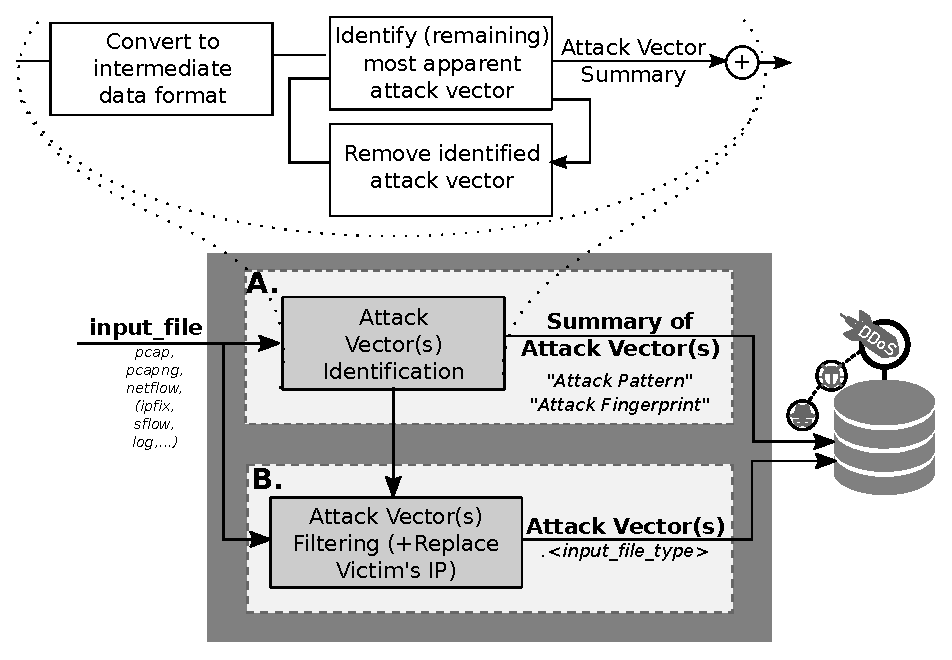
\includegraphics[width=0.5\textwidth]{{figs/ddos_fingerprinting.eps}}
	\caption{Process overview of the DDoS Dissector attack vector extraction}
\end{figure}







 

\section{DDoS Fingerprint Converters}
\label{sec:fingerprint_converters}

\section{The DDoSDB}
\label{sec:ddosdb}

More than a database with DDoS attack fingerprints.


Requirements:
\begin{itemize}
	\item flexible regarding the number and types of fields; 
	\item flexible access control
	\item distributed fashion;
	\item enrich the fingerprint;
	\item facilitate queries;
	\item enable download of fingerprints and anonymized data;
	\item facilitate notification;
	\item distribute information;
	\item upload information from only from trusted parties;
\end{itemize}

The aim of DDoSDB is twofold. On the one hand, it can help to create proactive measures of defying DDoS attacks, or recognise them in a very early stage. On the other hand, it can help us link the origin of multiple independent attacks together, thereby aiding law enforcement in the apprehending of the perpetrator. 

As stated in \ref{sec:ddos_dissector}, 
\section{DDoS Clearing House}
\label{sec:ddos_clearinghouse}

\subsection{Risks of running a version of DDoSDB}

\begin{itemize}
	\item Input normal network measurement (in case ops_team analyze flash crowd)
	\item Data leakage on the `user database’ (malicious access and upload)
	\item Data leakage on the `fingerprint database’;
	\item Data leakage on the `filtered and annonymized network measurements’;
	\item Data leakage of the `logs';
	\item Ill-intentioned users.
\end{itemize}


\section{Conclusion and Future Work}

DDoS attacks are not likely to stop occurring. However, we strongly believe that an community effort would extinguish the 

Would be very interesting DDoSDB being a target of DDoS attack. In this way, we could get new attacks, because old attacks are not supposed to take us down.
%------------------------------------------------------------------------------
% BIBLIOGRAPHY
%-------------------------------------------------------------------------------
%\bibliographystyle{ACM-Reference-Format-num}
\bibliographystyle{unsrtnat} %abbrvnat OR unsrtnat OR plainnat
\bibliography{reference}
%-------------------------------------------------------------------------------
\section*{Acknowledgements}

The ideas in this document were originally funded, in 2017, by SIDNfonds (an independent foundation established by the .nl ccTLD), then in 2018, these ideas were embraced by a coalition of 25 Dutch players from industry (ISPs, xSPs,IXPs, banks, not-for-profit DDoS protection providers) and gov’t (ministries and agencies), facilitated by Dutch National Cyber Security Centre (NCSC-NL), and, in 2019, it got funded by the European Commission in a project involving 46 partners.
\end{document}